\chapter{Avancement général}
\label{chapter1}

Ci-dessous un diagramme représentant l'avancement des différentes taches du projet. Le gris indique qu'une tache est terminée ou à un niveau d'avancement satisfaisant et garantissant une maturité proche. Le orange indique qu'une tache est particulièrement urgente ou critique pour le projet.

\begin{figure}[H]
    \centering
	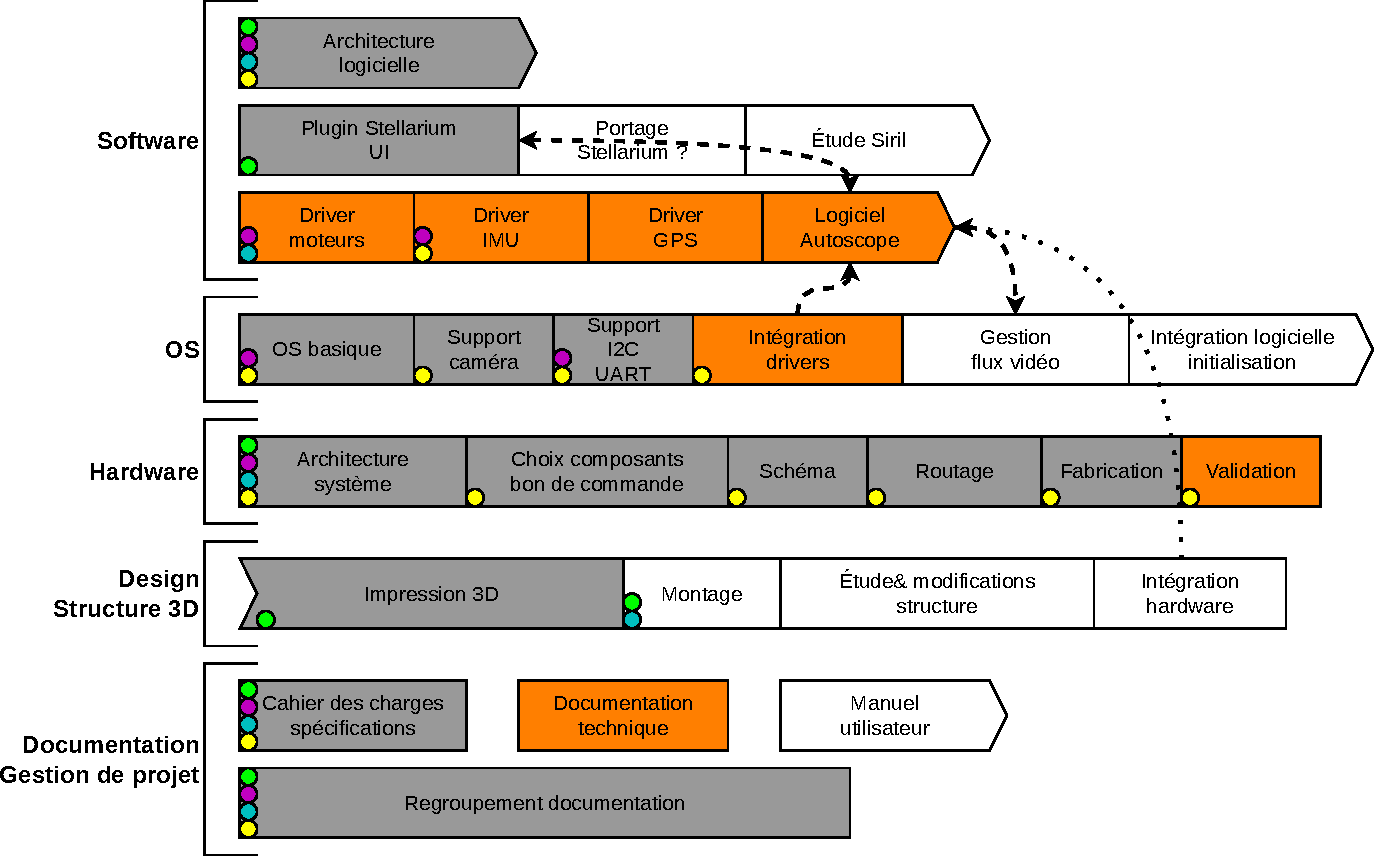
\includegraphics[width=1\linewidth]{\figures/sch_gantt.pdf}
    \decoRule
    \caption[
    Diagramme de l'organisation temporelle du travail sur le projet]{
    Diagramme de l'organisation temporelle du travail sur le projet}
    \label{fig:Diagramme de l'organisation temporelle du travail sur le projet}
    \end{figure}


